{
\metroset{titleformat frame=smallcaps}
\begin{frame}{Use Case 2: Wire-Speed DDoS Defense}
\vspace{6pt}
  \subtitlebar{Lightweight ML at the data plane eliminates controller-based reaction lag}

  \begin{columns}[T, totalwidth=\textwidth]

    % ── Left: 3 Boxes ─────────────────────────────────────
    \begin{column}{0.44\textwidth}

      \begin{tcolorbox}[problemcard=problemred]
        {\color{problemred}\bfseries\scriptsize The Threat}\\[2pt]
        {\footnotesize\color{HUAdark}
          DDoS attacks flood the network with
          massive traffic, aiming to overwhelm
          and paralyze the central controller.}
      \end{tcolorbox}

      \vspace{6pt}

      \begin{tcolorbox}[problemcard=HUAblue]
        {\color{HUAblue}\bfseries\scriptsize AI in Action}\\[2pt]
        {\footnotesize\color{HUAdark}
          Lightweight ML models analyze packet
          features locally (IP, UDP, TCP, SYN
          counts) and classify traffic in real time.}
      \end{tcolorbox}

      \vspace{6pt}

      \begin{tcolorbox}[problemcard=solutiongreen]
        {\color{solutiongreen}\bfseries\scriptsize PDP Result}\\[2pt]
        {\footnotesize\color{HUAdark}
          Malicious packets are dropped directly
          at the switch --- no controller round-trip,
          no attack reaches the server.}
      \end{tcolorbox}

    \end{column}

    % ── Vertical Divider ─────────────────────────────────
    \begin{column}{0.02\textwidth}
      \centering
      \textcolor{HUAlight}{\rule{0.5pt}{0.83\textheight}}
    \end{column}

    % ── Right: Fig. 6 ────────────────────────────────────
    \begin{column}{0.45\textwidth}
      \centering
      \vspace{0.15cm}
      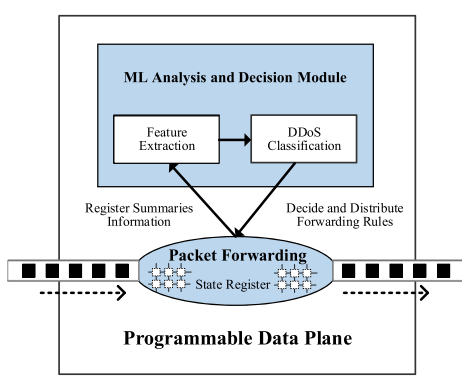
\includegraphics[width=\textwidth]{figures/fig6.png}
      \vspace{0.15cm}
      \begin{tcolorbox}[
        enhanced, boxrule=0pt,
        colback=HUApale, colframe=HUApale,
        arc=3pt, left=5pt, right=5pt,
        top=2pt, bottom=2pt,
      ]
        \centering
        \scriptsize\color{HUAdark}\itshape
        Defending DDoS Attacks with AI and PDP
        %(Quan et al., Fig.~6)
      \end{tcolorbox}
    \end{column}

  \end{columns}

\end{frame}
}